\documentclass[10pt]{gulartcl}
\usepackage{../exstyle}

\title{Esercizio settimanale n. 3}
\author{Guglielmo Bordin}
\date{\today}

\begin{document}
\maketitle
    
\noindent
Quattro particelle cariche di massa $m$ e carica $q$, tre positive e una
negativa, sono poste ai vertici di un quadrato di lato $\ell$ come mostrato
in figura. La particella in alto a destra viene poi rilasciata, lasciando
le altre vincolate al loro posto. 
\begin{enumerate}
    \item Dove si dirigerà? Indicare la direzione come angolo rispetto
        all’orizzontale.
    \item Che velocità avrà quando si troverà a grandissima distanza dalle
        altre cariche?
\end{enumerate}

\bigbreak
\begin{center}
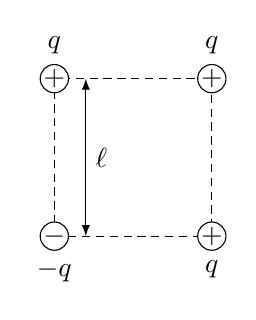
\begin{tikzpicture}
    \draw[densely dashed] (0, 0) -- (2, 0) -- (2, 2) -- (0, 2) -- cycle;
    \node[inner sep=0pt, circle, draw, fill=white, label={below:{$-q$}}]
        at (0, 0) {$-$};
    \node[inner sep=0pt, circle, draw, fill=white, label={below:{$q$}}]
        at (2, 0) {$+$};
    \node[inner sep=0pt, circle, draw, fill=white, label={above:{$q$}}]
        at (0, 2) {$+$};
    \node[inner sep=0pt, circle, draw, fill=white, label={above:{$q$}}]
        at (2, 2) {$+$};
    \draw[latex-latex] (0.4, 0) -- ++(0, 2) node[midway, anchor=west]
        {$\ell$};
\end{tikzpicture} 
\end{center}

\begin{solution}
I campi prodotti dalla carica in alto a sinistra e da quella in basso a
destra sono uguali in modulo, e diretti rispettivamente lungo il verso
positivo dell’asse $x$ e lungo il verso positivo dell’asse $y$. Il campo
risultante, che possiamo chiamare $\vec{E}_{+}$, ha espressione
\begin{equation}
    \vec{E}_{+} = \frac{q}{4\pi\epsilon_0 \ell^{2}} (\uvec{x} + \uvec{y}).
\end{equation}
Il campo prodotto dall’unica carica negativa ha invece modulo
\begin{equation}
    E_{-} = \frac{q}{8\pi\epsilon_0 \ell^{2}},
\end{equation}
poiché la distanza che separa la carica e il punto in cui stiamo valutando
il campo è, in questo caso, $\sqrt{2} \ell$, la diagonale del quadrato.
Per proiettare lungo $x$ e $y$ dobbiamo moltiplicare per $-\cos(\pi / 4) =
-1 / \sqrt{2}$, ottenendo
\begin{equation}
    \vec{E}_{-} = -\frac{q}{8\sqrt{2}\pi\epsilon_0 \ell^{2}} (\uvec{x} +
    \uvec{y}).
\end{equation}

Sommando $\vec{E}_{+}$ ed $\vec{E}_{-}$ otteniamo il campo prodotto
complessivamente dalle tre cariche,
\begin{equation}
    \vec{E} = \left(1 - \frac{\sqrt{2}}{4}\right) \frac{q}{4\pi\epsilon_0
    \ell^2} (\uvec{x} + \uvec{y}).
\end{equation}
Il prefattore numerico $1 - \sqrt{2} / 4 \approx \num{0.65}$ è positivo,
quindi il verso è positivo lungo la direzione individuata da $\uvec{x} +
\uvec{y}$, che è inclinata di \qty{45}{\degree} rispetto all’asse $x$. La
carica rilasciata è positiva: si muoverà pertanto lungo il verso positivo del
campo percepito, allontanandosi dal quadrato.

Per calcolare la velocità a grandissima distanza conviene ragionare sulla
conservazione dell’energia. La particella inizialmente è ferma, ma ha
un’energia potenziale dovuta all’interazione elettrostatica con le altre
tre particelle del quadrato. Aumentando la distanza l’interazione
elettrostatica diminuisce e l’energia potenziale iniziale viene convertita
in energia cinetica; la conversione sarà totale solo nel limite di distanza
infinita. Possiamo dunque scrivere l’equivalenza
\begin{equation}
    q V_{0} = \frac{1}{2} m v_{\infty}^{2},
    \label{eq:energy-cons}
\end{equation}
dove $V_0$ rappresenta il potenziale sentito dalla carica nella
configurazione iniziale, e $v_{\infty}$ la velocità raggiunta
all’infinito.

Per calcolare $V_{0}$ sommiamo i contributi delle altre tre cariche:
\begin{equation}
    V_0 = \frac{q}{4\pi\epsilon_0 \ell} + \frac{q}{4\pi\epsilon_0 \ell} -
    \frac{q}{4\pi\epsilon_0 (\sqrt{2}\ell)} = \left(\frac{4 - \sqrt{2}}{2}\right)
    \frac{q}{4\pi\epsilon_0 \ell}.
\end{equation}
Inserendo il risultato nell’equazione \eqref{eq:energy-cons} otteniamo
\begin{equation}
    \left(\frac{4 - \sqrt{2}}{\cancel{2}}\right) \frac{q^{2}}{4 \pi \epsilon_0 \ell}
    = \frac{1}{\cancel{2}} m v_{\infty}^{2},
\end{equation}
che porta all’espressione cercata
\begin{equation}
    v_{\infty} = \sqrt{\frac{(4 - \sqrt{2}) q^{2}}{4\pi\epsilon_0 m
    \ell}}.
\end{equation}
\end{solution}
\end{document}
